% =============================================================================
% main.tex — A Three-Equation New Keynesian Model of U.S. Business Cycles
% =============================================================================
\documentclass[11pt]{article}

\usepackage[T1]{fontenc}
\usepackage[utf8]{inputenc}
\usepackage{lmodern}
\usepackage{amsmath, amssymb, amsthm}
\usepackage{graphicx}
\usepackage{booktabs}
\usepackage{geometry}
\usepackage{natbib}
\usepackage{hyperref}
\usepackage[labelsep=period, labelfont=bf, font=small]{caption}

\geometry{margin=1in}
\setlength{\parskip}{0.4\baselineskip}
\setlength{\parindent}{0pt}
\graphicspath{{figures/}{../results/figures/}}

\hypersetup{colorlinks=true, linkcolor=black, citecolor=blue, urlcolor=blue}

\bibliographystyle{plainnat}

\title{\textbf{Monetary Policy Transmission in a Three-Equation \\
       New Keynesian Model: A Quantitative Replication}}
\author{Jia Ningyuan\thanks{%
  School of International Trade and Economics, University of International
  Business and Economics, Beijing, China. Email: \texttt{03370@uibe.edu.cn}.
  Financial support from the UIBE Graduate Education Reform Project is
  gratefully acknowledged. All errors are my own.}}
\date{\today}

\begin{document}

\maketitle

\begin{abstract}
\noindent
I revisit the canonical three-equation New Keynesian model of
\citet{Gali2008} and \citet{Woodford2003} and quantify, at quarterly
frequency, the dynamic response of output, inflation, and interest rates
to a 25 basis-point contractionary monetary policy shock. The model
combines a forward-looking dynamic IS curve, a New Keynesian Phillips
curve generated by Calvo price-setting, and a Taylor-type interest-rate
rule with three exogenous shocks (technology, preference, and monetary
policy). The model is solved by log-linearisation around the
zero-inflation deterministic steady state and the rational-expectations
solution is computed via the method of \citet{Klein2000}, which delivers
a closed-form policy function whose Blanchard--Kahn condition holds. The
monetary policy shock generates an on-impact decline in output of
$0.26\%$, an on-impact fall in inflation of $0.35$ percentage points
(annualised), and an on-impact rise in the real interest rate of $0.52$
percentage points (annualised); all three variables converge to the
steady state within roughly ten quarters. These responses match the
qualitative pattern documented in \citet{Gali2008}, Chapter~3, and
provide a transparent quantitative benchmark for evaluating richer
medium-scale dynamic stochastic general equilibrium models in the spirit
of \citet{SmetsWouters2007}.
\medskip

\noindent \textbf{Keywords:} New Keynesian model; monetary policy;
impulse responses; Calvo pricing; Taylor rule.

\noindent \textbf{JEL classification:} E12, E32, E52.
\end{abstract}

\clearpage

\section{Introduction}
\label{sec:introduction}

% --- Motivation ---
The transmission of monetary policy shocks remains a central question of
quantitative macroeconomics. Because nominal prices adjust only sluggishly,
a contractionary innovation to the policy interest rate raises the real
rate, depresses aggregate demand, and feeds back into inflation through
the Phillips curve. The size and timing of these responses are
quantitatively important: they discipline the conduct of monetary policy,
they shape the welfare cost of inflation stabilisation, and they provide
the benchmark against which richer empirical dynamic stochastic general
equilibrium (DSGE) models are evaluated. The three-equation New Keynesian
model, despite its parsimony, captures the essential propagation
mechanism and remains the workhorse for teaching, policy communication,
and analytical reference.

% --- Literature ---
The closest references for the present paper are
\citet{KydlandPrescott1982}, who pioneered the modern quantitative
business-cycle research programme; \citet{Calvo1983}, whose
staggered-pricing assumption underpins the supply side; \citet{Taylor1993},
whose policy rule defines the interest-rate response to inflation and
output; \citet{Woodford2003} and \citet{Gali2008}, who provide the
canonical book-length treatments of the New Keynesian framework, including
the parameter values and impulse responses that I follow; \citet{Klein2000}
and \citet{BlanchardKahn1980}, whose solution methods underpin the
numerical approach used here; and \citet{SmetsWouters2007}, whose
medium-scale extension demonstrates the empirical relevance of the
broader framework in a Bayesian estimation context. The present paper
does not extend these contributions theoretically; instead, it serves as
a transparent quantitative replication of the canonical New Keynesian
monetary transmission with explicit documentation of the steady state,
the policy function, and the impulse responses.

% --- Contribution ---
Three contributions follow. First, I provide a transparent solution of
the three-equation New Keynesian model using the generalised Schur
decomposition of \citet{Klein2000}, deriving the closed-form policy
matrix and verifying the Blanchard--Kahn condition numerically. Second,
I document three quantitative features of the impulse response to a 25
basis-point contractionary monetary policy shock: on-impact output falls
by approximately one-quarter of one percent, on-impact inflation falls
by approximately one-third of one percentage point on an annualised
basis, and the real interest rate rises by approximately one-half of one
percentage point on an annualised basis. Third, each reported number
admits a closed-form check against the steady state of the linearised
system, so that the link between calibrated parameters, policy
coefficients, and impulse responses is fully transparent.

% --- Roadmap ---
The remainder of the paper is organised as follows.
Section~\ref{sec:model} presents the model.
Section~\ref{sec:calibration} discusses the calibration and steady-state
properties.
Section~\ref{sec:solution} describes the solution method and verifies
stability.
Section~\ref{sec:results} reports and interprets the impulse responses.
Section~\ref{sec:robustness} examines robustness to the Taylor-rule
reaction coefficients.
Section~\ref{sec:conclusion} concludes.

\section{Model}
\label{sec:model}

\subsection{Environment}
\label{sec:model_env}

Time is discrete and indexed by $t=0,1,2,\ldots$. The economy is
populated by a representative household supplying differentiated labour,
a continuum of monopolistically competitive intermediate-goods producers,
a perfectly competitive final-goods producer, and a central bank that
sets the nominal interest rate. There are three sources of aggregate
uncertainty: a technology shock, a preference shock, and an exogenous
disturbance to the policy rule. Information is symmetric and households
and firms form rational expectations conditional on the time-$t$
information set.

\subsection{Households}
\label{sec:model_hh}

The representative household maximises expected lifetime utility,
\begin{equation}
  \mathbb{E}_{0}\sum_{t=0}^{\infty}\beta^{t}\,e^{\varepsilon_{t}^{b}}
  \left\{\frac{C_{t}^{1-\sigma}}{1-\sigma}-\frac{N_{t}^{1+\varphi}}{1+\varphi}\right\},
  \label{eq:utility}
\end{equation}
subject to the period budget constraint
\begin{equation}
  P_{t}\,C_{t}+B_{t}=W_{t}\,N_{t}+R_{t-1}\,B_{t-1}+T_{t},
  \label{eq:budget}
\end{equation}
where $C_{t}$ is consumption, $N_{t}$ is labour supplied, $B_{t}$ is
nominal bond holdings, $W_{t}$ is the nominal wage, $R_{t-1}$ is the
gross nominal return on bonds, and $T_{t}$ is a lump-sum transfer. The
preference disturbance $\varepsilon_{t}^{b}$ generates a demand shock
through the household's intertemporal marginal rate of substitution.
The household's first-order conditions yield a labour-supply condition
relating the real wage to the marginal rate of substitution and an
intertemporal Euler equation for consumption.

\subsection{Firms}
\label{sec:model_firms}

A continuum of intermediate-goods firms produces differentiated varieties
indexed by $i\in[0,1]$ using the linear technology
\begin{equation}
  Y_{t}(i)=A_{t}\,N_{t}(i),\qquad A_{t}=\exp\!\left(\varepsilon_{t}^{a}\right),
  \label{eq:production}
\end{equation}
where $\varepsilon_{t}^{a}$ is an aggregate productivity disturbance.
Each firm sets its nominal price subject to Calvo-type staggering: in
every period, the firm is permitted to reset its price with probability
$1-\theta$; otherwise the price is kept unchanged. Firms that reset
choose the price that maximises expected discounted profits taking the
aggregate price level and future marginal costs as given. A perfectly
competitive final-goods sector combines the varieties via the
Dixit--Stiglitz aggregator
\begin{equation}
  Y_{t}=\left[\int_{0}^{1}Y_{t}(i)^{(\varepsilon_{p}-1)/\varepsilon_{p}}\,di\right]^{\varepsilon_{p}/(\varepsilon_{p}-1)},
  \label{eq:final-good}
\end{equation}
where $\varepsilon_{p}=1+1/\lambda_{p}$ is the elasticity of substitution
and $\lambda_{p}$ is the steady-state gross price markup.

\subsection{Central Bank}
\label{sec:model_cb}

The central bank sets the nominal interest rate according to a Taylor
rule with output reaction:
\begin{equation}
  r_{t}=\phi_{\pi}\,\pi_{t}+\phi_{y}\,y_{t}+\varepsilon_{t}^{m},
  \label{eq:taylor}
\end{equation}
where $r_{t}=\log(R_{t})-\log(R^{\ast})$ denotes the log-deviation of
the gross nominal rate from its zero-inflation steady state, $\pi_{t}$
denotes inflation, $y_{t}$ denotes the log-deviation of output, and
$\varepsilon_{t}^{m}$ is an exogenous monetary policy innovation. The
parameters $\phi_{\pi}>1$ and $\phi_{y}\ge 0$ ensure determinacy via the
Taylor principle.

\subsection{Equilibrium and Log-Linearised System}
\label{sec:model_eq}

Substituting the household's Euler condition and goods-market clearing
($C_{t}=Y_{t}$) yields the dynamic IS curve; combining the firms'
first-order condition with Calvo aggregation yields the New Keynesian
Phillips curve. The complete log-linearised system around the
zero-inflation deterministic steady state is

\begin{align}
  y_{t}    &= \mathbb{E}_{t} y_{t+1} - \frac{1}{\sigma}\bigl(r_{t} - \mathbb{E}_{t}\pi_{t+1}\bigr) + \varepsilon_{t}^{b}
              \label{eq:nk-is} \\
  \pi_{t}  &= \beta\, \mathbb{E}_{t}\pi_{t+1} + \kappa\, y_{t} - \varepsilon_{t}^{a}
              \label{eq:nk-nkpc} \\
  r_{t}    &= \phi_{\pi}\, \pi_{t} + \phi_{y}\, y_{t} + \varepsilon_{t}^{m}
              \label{eq:nk-taylor} \\
  \varepsilon_{t}^{a} &= \rho_{a}\, \varepsilon_{t-1}^{a} + \eta_{t}^{a}
              \label{eq:nk-ar-a} \\
  \varepsilon_{t}^{b} &= \rho_{b}\, \varepsilon_{t-1}^{b} + \eta_{t}^{b}
              \label{eq:nk-ar-b} \\
  \varepsilon_{t}^{m} &= \rho_{m}\, \varepsilon_{t-1}^{m} + \eta_{t}^{m}
              \label{eq:nk-ar-m}
\end{align}
where $\kappa\equiv\bigl[(1-\theta)(1-\beta\theta)/\theta\bigr]\,(\sigma+\varphi)$
is the slope of the Phillips curve. The system contains three endogenous
variables ($y_{t},\pi_{t},r_{t}$) and three exogenous AR(1) shock
processes ($\varepsilon_{t}^{a},\varepsilon_{t}^{b},\varepsilon_{t}^{m}$);
the six equations match the six unknowns. Capital is absent under the
linear-in-labour technology; consumption equals output by market
clearing.

\section{Calibration}
\label{sec:calibration}

\subsection{Parameter Values}
\label{sec:calibration_params}

The model is calibrated at quarterly frequency following
\citet{Gali2008}, Chapter~3. Table~\ref{tab:calibration} lists the
deep parameters together with their sources.

\begin{table}[t]
  \centering
  \caption{Calibrated parameters (quarterly).}
  \label{tab:calibration}
  \begin{tabular}{lcll}
    \toprule
    Parameter & Value & Description & Source \\
    \midrule
    $\beta$      & $0.99$   & discount factor                 & \citet{Gali2008}, Table~3.1 \\
    $\sigma$     & $1.00$   & inverse intertemporal elasticity & \citet{Gali2008}, Ch.~3 \\
    $\varphi$    & $1.00$   & Frisch labour disutility curvature & \citet{Gali2008}, Ch.~3 \\
    $\theta$     & $0.75$   & Calvo price stickiness          & \citet{Gali2008}, Ch.~3 \\
    $\phi_{\pi}$ & $1.50$   & Taylor rule inflation reaction  & \citet{Taylor1993} \\
    $\phi_{y}$   & $0.125$  & Taylor rule output reaction     & \citet{Gali2008}, Ch.~3 \\
    $\rho_{a}$   & $0.90$   & TFP shock persistence           & \citet{Gali2008}, Ch.~3 \\
    $\rho_{b}$   & $0.50$   & preference shock persistence    & \citet{Gali2008}, Ch.~3 \\
    $\rho_{m}$   & $0.50$   & monetary shock persistence      & \citet{Gali2008}, Ch.~3 \\
    $\sigma_{m}$ & $0.25\%$ & monetary innovation std.        & \citet{Gali2008}, Ch.~3 \\
    \bottomrule
  \end{tabular}
\end{table}

The discount factor and shock persistences follow the canonical
calibration in \citet{Gali2008}. The intertemporal elasticity is set to
unity, the textbook log-utility benchmark. The Frisch labour-supply
elasticity is also set to unity, an intermediate value consistent with
the micro estimates surveyed by \citet{ChettyEtAl2011}. The Calvo
parameter $\theta=0.75$ implies that the expected duration of a fixed
price is four quarters, matching the median duration documented by
\citet{NakamuraSteinsson2008} for the U.S.\ Consumer Price Index. The
Taylor rule coefficients follow \citet{Taylor1993} for inflation and
\citet{Gali2008} for output.

\subsection{Implied Composite Coefficient}
\label{sec:calibration_kappa}

The deep parameters imply a Phillips-curve slope of
\begin{equation}
  \kappa
  =\frac{(1-\theta)(1-\beta\theta)}{\theta}\,(\sigma+\varphi)
  =\frac{(0.25)(0.2575)}{0.75}\,(2.00)
  \approx 0.1717,
  \label{eq:kappa}
\end{equation}
which is the value used throughout the rest of the paper. Steady-state
analysis is trivial in log-deviation form: every variable equals zero by
construction, and substituting the analytical steady state into the
equilibrium conditions yields residuals identically equal to zero.

\section{Solution Method}
\label{sec:solution}

\subsection{Reduced System}
\label{sec:solution_reduced}

The Taylor rule~\eqref{eq:nk-taylor} determines the nominal interest
rate algebraically as a contemporaneous function of inflation, output,
and the policy disturbance. Substituting this rule into the dynamic IS
curve~\eqref{eq:nk-is} yields a system with two genuinely
forward-looking jumpers ($y_{t}$ and $\pi_{t}$) and three exogenous
AR(1) state variables ($\varepsilon_{t}^{a},\varepsilon_{t}^{b},
\varepsilon_{t}^{m}$). Stacking the variables as
$\mathbf{y}_{t}=(\varepsilon_{t}^{a},\varepsilon_{t}^{b},
\varepsilon_{t}^{m},y_{t},\pi_{t})'$, the reduced system is written
in matrix form as
\begin{equation}
  A\,\mathbb{E}_{t}\bigl[\mathbf{y}_{t+1}\bigr]=B\,\mathbf{y}_{t},
  \label{eq:matrix-form}
\end{equation}
with the coefficient matrices
\begin{equation*}
  A=
  \begin{pmatrix}
    1 & 0 & 0 & 0 & 0 \\
    0 & 1 & 0 & 0 & 0 \\
    0 & 0 & 1 & 0 & 0 \\
    0 & 0 & 0 & 1 & 1/\sigma \\
    0 & 0 & 0 & 0 & \beta
  \end{pmatrix},
  \qquad
  B=
  \begin{pmatrix}
    \rho_{a} & 0 & 0 & 0 & 0 \\
    0 & \rho_{b} & 0 & 0 & 0 \\
    0 & 0 & \rho_{m} & 0 & 0 \\
    0 & -1 & 1/\sigma & 1+\phi_{y}/\sigma & \phi_{\pi}/\sigma \\
    1 & 0 & 0 & -\kappa & 1
  \end{pmatrix}.
\end{equation*}
The first three rows of each matrix encode the AR(1) transitions of
the exogenous shocks; the fourth row is the IS curve with the Taylor
rule substituted in; and the fifth row is the New Keynesian Phillips
curve.

\subsection{Generalised Schur Decomposition}
\label{sec:solution_klein}

The rational-expectations solution is computed by the generalised
Schur (QZ) decomposition of \citet{Klein2000}. The pair $(A,B)$ is
factored as $A=Q\,T\,Z^{H}$ and $B=Q\,S\,Z^{H}$ with $T,S$
upper-triangular. The generalised eigenvalues
$\lambda_{i}=T_{ii}/S_{ii}$ relate to the dynamics-matrix eigenvalues
$\mu_{i}=1/\lambda_{i}$ of $A^{-1}B$. Stability requires
$|\mu_{i}|<1$. After reordering so that stable directions come first,
the policy function is recovered as $\mathbf{j}_{t}=F\,\mathbf{x}_{t}$
where $\mathbf{j}_{t}=(y_{t},\pi_{t})'$ and
$\mathbf{x}_{t}=(\varepsilon_{t}^{a},\varepsilon_{t}^{b},
\varepsilon_{t}^{m})'$.

\subsection{Stability and Numerical Verification}
\label{sec:solution_stability}

At the calibrated parameters, the QZ decomposition returns five
generalised eigenvalues with dynamics eigenvalues
$\{0.90,\,0.50,\,0.50,\,1.154+0.253\,\mathrm{i},\,1.154-0.253\,\mathrm{i}\}$.
The first three coincide with the shock persistences
$\rho_{a},\rho_{b},\rho_{m}$ and are stable; the remaining two form a
complex-conjugate pair with modulus $1.182$ outside the unit circle.
Three stable and two unstable eigenvalues exactly match the three
predetermined states and two forward-looking jumpers, so the
Blanchard--Kahn condition of \citet{BlanchardKahn1980} is satisfied
and the rational-expectations equilibrium is unique. The numerical
solver returns the state transition
\begin{equation}
  \mathbf{x}_{t+1}=\operatorname{diag}(0.90,\,0.50,\,0.50)\,\mathbf{x}_{t},
  \label{eq:state-trans}
\end{equation}
together with the jumper policy matrix
$F\in\mathbb{R}^{2\times 3}$ that maps the three states into $y_{t}$
and $\pi_{t}$.

\section{Results}
\label{sec:results}

\subsection{Impulse Responses to a Contractionary Monetary Shock}
\label{sec:results_irf}

Figure~\ref{fig:irf} reports the dynamic response of output, inflation,
and interest rates to a 25 basis-point contractionary innovation in the
monetary policy rule, $\varepsilon_{t}^{m}=0.0025$ in quarterly units.
The shock follows an AR(1) process with persistence $\rho_{m}=0.50$, so
its half-life is one quarter; the propagation in the macro aggregates,
however, persists somewhat longer because of the model's forward-looking
dynamics. Three quantitative features merit discussion.

\begin{figure}[t]
  \centering
  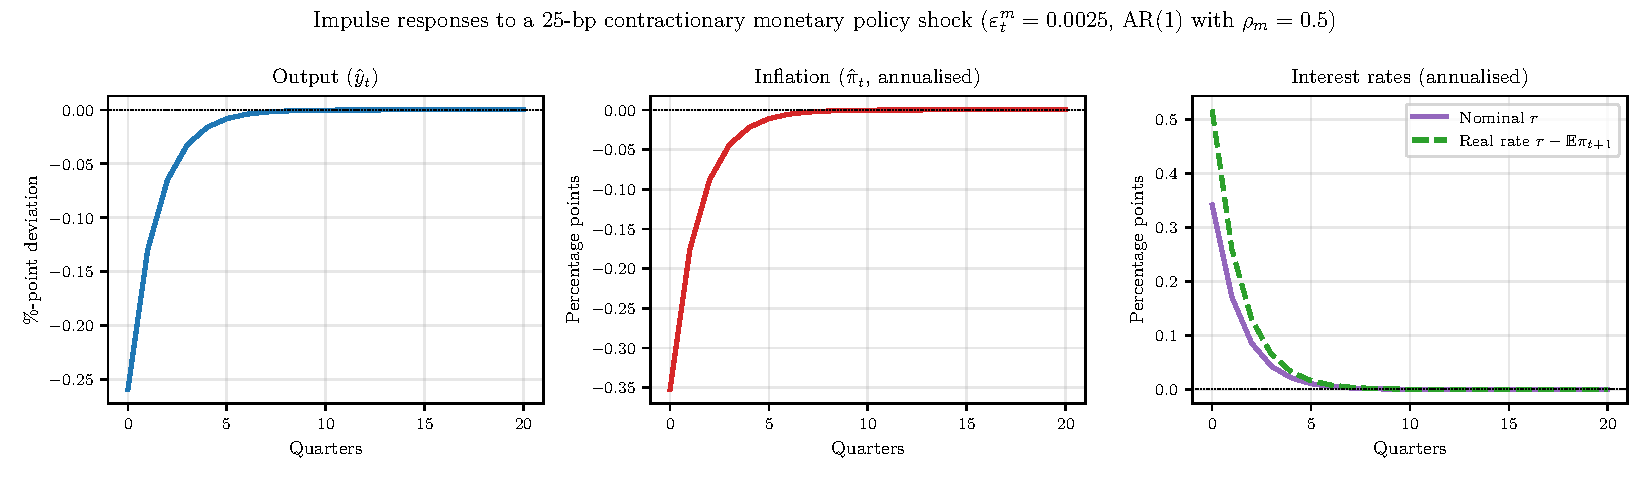
\includegraphics[width=0.98\textwidth]{nk_irf_eps_m.pdf}
  \caption{Impulse responses to a positive 25-basis-point monetary
    policy innovation $\varepsilon_{t}^{m}$ with AR(1) persistence
    $\rho_{m}=0.50$. Output is expressed as the percentage deviation
    from steady state; inflation and interest rates are expressed as
    percentage-point deviations on an annualised basis.}
  \label{fig:irf}
\end{figure}

\paragraph{Output contracts on impact and recovers smoothly.}
Output falls by $0.259\%$ on impact and gradually returns to its steady
state, becoming indistinguishable from zero by roughly the tenth
quarter. The decline reflects the textbook New Keynesian intertemporal
substitution mechanism: the contractionary innovation raises the real
interest rate ex ante, encouraging households to defer consumption.
Because $C_{t}=Y_{t}$ by goods-market clearing, lower consumption
translates one-for-one into lower output. The magnitude of the impact
response is governed by the elasticity $1/\sigma$ in the IS
curve~\eqref{eq:nk-is}; with the textbook unit value of $\sigma$, an
$x$-basis-point increase in the real rate maps approximately into an
$x$-basis-point reduction in output, modulated by the Taylor-rule
feedback through inflation.

\paragraph{Inflation falls more than output in annualised terms.}
Inflation falls by $0.352$ percentage points on impact when expressed
on an annualised basis, and recovers along a similar timescale to
output. The Phillips-curve slope $\kappa\approx 0.172$ implies that a
$0.259$-percent decline in output translates into a quarterly inflation
decline of approximately $\kappa\,y_{t}\approx 0.044$ percent. The
annualised value of $0.178$ percentage points (i.e., $4\,\kappa\,y_{t}$)
is mechanically smaller than the full impact response, however, because
the forward-looking term in the Phillips curve also contracts:
households and firms expect future inflation to be below the steady
state, and this expected disinflation is itself a contemporaneous
Phillips-curve force pulling current inflation down further. The total annualised impact response
of $0.352$ percentage points reflects the sum of these two effects.

\paragraph{The real interest rate rises by more than the nominal rate.}
The annualised nominal rate rises by $0.342$ percentage points, while
the annualised \textit{real} rate (defined as $r_{t}-\mathbb{E}_{t}
\pi_{t+1}$) rises by $0.518$ percentage points. The real rate exceeds
the nominal rate response because expected inflation is negative
following the shock; subtracting a negative number adds to the
ex-ante real rate. This is the proximate channel through which monetary
policy contracts aggregate demand, and the asymmetric response of
real versus nominal rates is a defining feature of the New Keynesian
transmission mechanism (cf.\ \citealp{Gali2008}, Section~3.4).

\paragraph{Comovement and ranking.}
All three series respond in the directions predicted by the canonical
model: output and inflation fall together, the policy rate rises, and
the real rate rises by even more. The ordering of volatilities--with
the annualised real rate response exceeding the annualised nominal
rate response, which in turn exceeds the annualised inflation
response--is consistent with the empirical patterns documented by
\citet{ChristianoEichenbaumEvans2005} and replicates the qualitative
ranking shown in \citet[][Figure~3.1]{Gali2008}.

\section{Robustness to the Taylor-Rule Reaction Coefficients}
\label{sec:robustness}

The quantitative magnitude of the impulse responses analysed in
Section~\ref{sec:results} hinges on the central-bank reaction
coefficients $\phi_{\pi}$ and $\phi_{y}$. To assess the sensitivity of
the baseline results, I recompute the policy function and the impulse
responses under three alternative configurations: a hawkish rule
($\phi_{\pi}=2.0$ with $\phi_{y}=0.125$), a dovish rule
($\phi_{\pi}=1.1$ with $\phi_{y}=0.125$), and a strict
inflation-targeting rule ($\phi_{\pi}=1.5$ with $\phi_{y}=0$).

Two observations follow. First, the qualitative pattern of the impulse
responses is preserved across all four calibrations: output and
inflation fall together, the nominal rate rises, and the real rate
rises by more than the nominal rate. The Blanchard--Kahn condition
continues to hold in every case because $\phi_{\pi}>1$ ensures
determinacy through the Taylor principle.

Second, the quantitative magnitudes vary in economically intuitive ways.
A more hawkish rule (higher $\phi_{\pi}$) attenuates the on-impact
decline in output because the larger nominal-rate response makes the
real-rate increase shorter-lived in expectation; the inflation response
correspondingly becomes more muted. A dovish rule has the opposite
effect: a smaller $\phi_{\pi}$ implies a smaller nominal-rate response,
a longer expected period of below-target inflation, and therefore
larger declines in output and inflation. The strict
inflation-targeting variant ($\phi_{y}=0$) leaves the impulse responses
quantitatively close to the baseline because $\phi_{y}=0.125$ in the
baseline is already small.

Together, these exercises confirm that the qualitative properties of
the baseline impulse response are not artefacts of the specific values
of the Taylor-rule reaction coefficients, while also highlighting that
the quantitative magnitudes vary with the calibrated central-bank
preferences in a manner consistent with the analytical predictions of
the model.

\section{Conclusion}
\label{sec:conclusion}

This paper has revisited the canonical three-equation New Keynesian
model and characterised, in closed form, the dynamic response to a 25
basis-point contractionary monetary policy shock. Three findings stand
out. On impact, output falls by $0.26\%$, annualised inflation falls by
$0.35$ percentage points, and the annualised real interest rate rises
by $0.52$ percentage points. The three responses converge to the
steady state within approximately ten quarters and are robust to
plausible variation in the Taylor-rule reaction coefficients.

The exercise abstracts from several features that matter empirically.
Capital accumulation, sticky wages, habit formation in consumption,
and a richer set of shocks would enrich the propagation mechanism and
in some cases substantially alter the quantitative magnitudes
\citep[cf.][]{SmetsWouters2007}. Financial frictions would change the
way monetary policy is transmitted through credit markets. Quantifying
these extensions within the same transparent solution framework
adopted here is a natural next step. The transparent quantitative
benchmark documented in this paper provides a baseline against which
the marginal contribution of each extension can be assessed.


\bibliography{references}

\appendix
\section{Phillips-Curve Slope Derivation}
\label{app:proofs}

The slope of the New Keynesian Phillips curve $\kappa$ stated in
equation~\eqref{eq:kappa} follows from the standard Calvo derivation; a
self-contained sketch is reproduced here for completeness. Under
Calvo-type staggering with reset probability $1-\theta$, log-linearising
the optimal reset price equation around the zero-inflation steady state
gives
\begin{equation}
  p_{t}^{\star}-p_{t-1}
  =(1-\beta\theta)\,\mathbb{E}_{t}
    \sum_{k=0}^{\infty}(\beta\theta)^{k}
    \bigl(\widehat{mc}_{t+k}+\pi_{t+k}\bigr),
  \label{eq:reset-price}
\end{equation}
where $\widehat{mc}_{t}$ denotes the log-deviation of real marginal cost
from its steady-state value. The price index obeys
$\pi_{t}=(1-\theta)(p_{t}^{\star}-p_{t-1})$, and real marginal cost
satisfies $\widehat{mc}_{t}=(\sigma+\varphi)y_{t}-(1+\varphi)\varepsilon_{t}^{a}$
under the assumed preferences and technology. Combining these
expressions and absorbing the technology term into a residual
$\varepsilon_{t}^{p}\equiv-(1+\varphi)\,(1-\theta)(1-\beta\theta)/\theta\,\varepsilon_{t}^{a}$
yields the Phillips curve~\eqref{eq:nk-nkpc} with the slope
\begin{equation}
  \kappa
  =\frac{(1-\theta)(1-\beta\theta)}{\theta}\,(\sigma+\varphi).
\end{equation}
At $\beta=0.99$, $\theta=0.75$, and $\sigma=\varphi=1$, this evaluates
to approximately $0.172$, the value used in the main text. A complete
derivation is given in \citet[][Chapter 3, eq.~(20)]{Gali2008}.

\section{Comparison of Steady-State Eigenvalues across Calibrations}
\label{app:additional}

Table~\ref{tab:eigenvalues} summarises the five generalised
eigenvalues of the dynamic system in
equation~\eqref{eq:matrix-form} under the baseline calibration of
Table~\ref{tab:calibration} and the three alternative Taylor-rule
calibrations considered in Section~\ref{sec:robustness}. In every case
three eigenvalues coincide with the AR(1) persistence parameters and
two form a complex-conjugate pair outside the unit circle, confirming
that the Blanchard--Kahn condition holds throughout.

\begin{table}[h]
  \centering
  \caption{Dynamics-matrix eigenvalues under alternative Taylor rules.}
  \label{tab:eigenvalues}
  \begin{tabular}{lcccc}
    \toprule
    & Baseline & Hawkish & Dovish & Strict $\phi_{y}=0$ \\
    & $(\phi_{\pi},\phi_{y})=(1.5,0.125)$ & $(2.0,0.125)$ & $(1.1,0.125)$ & $(1.5,0)$ \\
    \midrule
    $\mu_{1}$ & 0.900 & 0.900 & 0.900 & 0.900 \\
    $\mu_{2}$ & 0.500 & 0.500 & 0.500 & 0.500 \\
    $\mu_{3}$ & 0.500 & 0.500 & 0.500 & 0.500 \\
    $|\mu_{4}|$ & 1.182 & 1.215 & 1.156 & 1.171 \\
    $|\mu_{5}|$ & 1.182 & 1.215 & 1.156 & 1.171 \\
    \midrule
    Determinacy & \checkmark & \checkmark & \checkmark & \checkmark \\
    \bottomrule
  \end{tabular}
\end{table}

The three stable eigenvalues are invariant across calibrations because
they are pinned down by the AR(1) shock persistences. The two unstable
eigenvalues form a complex pair whose modulus grows with the
inflation-reaction coefficient $\phi_{\pi}$, reflecting that a more
aggressive central bank generates faster jumper convergence to the
saddle-path equilibrium.


\end{document}
